\section{函数的 Fourier 级数}

\begin{problem}{Fourier级数展开}{Fourier-Series-Expansion}
    作出下列周期 $2\uppi$ 的函数的图形，并把它们展开成 Fourier 级数（说明收敛情况）．
    \begin{enumerate}
        \item 在 $[-\uppi, \uppi)$ 中， $f(x) = \begin{dcases} -\uppi, & -\uppi \leqslant x \leqslant 0, \\ x, & 0 < x < \uppi; \end{dcases}$
        \item 在 $[-\uppi, \uppi)$ 中， $f(x) = \cos \frac{x}{2}$;
        \item 在 $[-\uppi, \uppi)$ 中， $f(x) = \begin{dcases} \e^x, & -\uppi \leqslant x \leqslant 0, \\ 1, & 0 \leqslant x < \uppi. \end{dcases}$
    \end{enumerate}
\end{problem}

\begin{solution}
    \ansitem{1}

    图形如下：
    \begin{center}
        \begin{tikzpicture}[scale=0.8]
            \draw[->] (-7,0) -- (7,0) node[right] {$x$};
            \draw[->] (0,-4.5) -- (0,4.5) node[above] {$y$};

            \draw[dashed] (-3.1416,-3.1416) -- (-3.1416,3.1416);
            \draw[dashed] (3.1416,-3.1416) -- (3.1416,3.1416);

            \node[below left] at (0,0) {$0$};
            \node[below] at (3.1416,0) {$\uppi$};
            \node[below] at (-3.1416,0) {$-\uppi$};
            \node[below] at (6.2832,0) {$2\uppi$};
            \node[below] at (-6.2832,0) {$-2\uppi$};

            % Period -1: [-2pi, -pi)
            \draw[thick, blue] (-6.2832, 0) -- (-3.1416, 3.1416);
            \draw[fill=white, draw=blue, thick] (-3.1416, 3.1416) circle (2pt);
            \draw[fill=white, draw=blue, thick] (-6.2832, 0) circle (2pt);
            \draw[fill=blue] (-6.2832, -3.1416) circle (2pt);

            % Period 0: [-pi, 0]
            \draw[thick, blue] (-3.1416, -3.1416) -- (0, -3.1416);
            \draw[fill=blue] (-3.1416, -3.1416) circle (2pt);
            \draw[fill=blue] (0, -3.1416) circle (2pt);

            % Period 0: (0, pi)
            \draw[thick, blue] (0, 0) -- (3.1416, 3.1416);
            \draw[fill=white, draw=blue, thick] (0, 0) circle (2pt);
            \draw[fill=white, draw=blue, thick] (3.1416, 3.1416) circle (2pt);

            % Period 1: [pi, 2pi]
            \draw[thick, blue] (3.1416, -3.1416) -- (6.2832, -3.1416);
            \draw[fill=blue] (3.1416, -3.1416) circle (2pt);
            \draw[fill=blue] (6.2832, -3.1416) circle (2pt);

            % Period 1: (2pi, 3pi)
            \draw[thick, blue] (6.2832, 0) -- (7, 0.7168);
            \draw[fill=white, draw=blue, thick] (6.2832, 0) circle (2pt);
        \end{tikzpicture}
    \end{center}

    计算 Fourier 系数：
    \begin{equation}
        \begin{aligned}
            a_0 & = \frac{1}{\uppi} \int_{-\uppi}^{\uppi} f(x) \d x                                          \\
                & = \frac{1}{\uppi} \left[ \int_{-\uppi}^{0} (-\uppi) \d x + \int_{0}^{\uppi} x \d x \right] \\
                & = \frac{1}{\uppi} \left[ -\uppi^2 + \frac{\uppi^2}{2} \right] = -\frac{\uppi}{2},
        \end{aligned}
    \end{equation}

    \begin{equation}
        \begin{aligned}
            a_n & = \frac{1}{\uppi} \int_{-\uppi}^{\uppi} f(x) \cos(nx) \d x                                                                      \\
                & = \frac{1}{\uppi} \left[ \int_{-\uppi}^{0} (-\uppi) \cos(nx) \d x + \int_{0}^{\uppi} x \cos(nx) \d x \right]                    \\
                & = \frac{1}{\uppi} \left[ 0 + \left. \frac{x \sin(nx)}{n} \right|_{0}^{\uppi} - \int_{0}^{\uppi} \frac{\sin(nx)}{n} \d x \right] \\
                & = \frac{(-1)^n - 1}{\uppi n^2},
        \end{aligned}
    \end{equation}

    \begin{equation}
        \begin{aligned}
            b_n & = \frac{1}{\uppi} \int_{-\uppi}^{\uppi} f(x) \sin(nx) \d x                                                                                                                         \\
                & = \frac{1}{\uppi} \left[ \int_{-\uppi}^{0} (-\uppi) \sin(nx) \d x + \int_{0}^{\uppi} x \sin(nx) \d x \right]                                                                       \\
                & = \frac{1}{\uppi} \left[ \left. \frac{\uppi \cos(nx)}{n} \right|_{-\uppi}^{0} - \left. \frac{x \cos(nx)}{n} \right|_{0}^{\uppi} + \int_{0}^{\uppi} \frac{\cos(nx)}{n} \d x \right] \\
                & = \frac{1}{\uppi} \left[ \frac{\uppi(1 - (-1)^n)}{n} - \frac{\uppi(-1)^n}{n} \right] = \frac{1 - 2(-1)^n}{n}.
        \end{aligned}
    \end{equation}

    因此，函数的 Fourier 展开式为
    \begin{equation}
        \boxed{f(x) \sim -\frac{\uppi}{4} + \sum_{n=1}^{\infty} \left[ \frac{(-1)^n - 1}{\uppi n^2} \cos(nx) + \frac{1 - 2(-1)^n}{n} \sin(nx) \right]}.
    \end{equation}

    收敛情况：由于 $f(x)$ 周期延拓后在 $[-\uppi, \uppi)$ 上分段光滑，由 Dirichlet 收敛定理，当 $x \neq k\uppi$ ($k \in \symbb{Z}$) 时，级数收敛于 $f(x)$；当 $x = 2k\uppi$ 时，级数收敛于 $-\frac{\uppi}{2}$；当 $x = (2k+1)\uppi$ 时，级数收敛于 $0$．

    \ansitem{2}

    图形如下：
    \begin{center}
        \begin{tikzpicture}[scale=0.8]
            \draw[->] (-7,0) -- (7,0) node[right] {$x$};
            \draw[->] (0,-0.5) -- (0,2.5) node[above] {$y$};

            \draw[dashed] (-3.1416,0) -- (-3.1416,1);
            \draw[dashed] (3.1416,0) -- (3.1416,1);

            \node[below left] at (0,0) {$0$};
            \node[below] at (3.1416,0) {$\uppi$};
            \node[below] at (-3.1416,0) {$-\uppi$};
            \node[below] at (6.2832,0) {$2\uppi$};
            \node[below] at (-6.2832,0) {$-2\uppi$};

            \draw[thick, blue, domain=-3.1416:3.1416, samples=100] plot (\x, {cos(\x*180/3.1416/2)});
            \draw[thick, blue, domain=3.1416:6.2832, samples=100] plot (\x, {cos((\x-6.2832)*180/3.1416/2)});
            \draw[thick, blue, domain=-6.2832:-3.1416, samples=100] plot (\x, {cos((\x+6.2832)*180/3.1416/2)});

            \node[left] at (0,1) {$1$};
            \draw[dashed] (0,1) -- (3.1416,1);
            \draw[fill=blue] (0,1) circle (2pt);
            \draw[fill=blue] (6.2832,1) circle (2pt);
            \draw[fill=blue] (-6.2832,1) circle (2pt);

            \draw[fill=blue] (3.1416,0) circle (2pt);
            \draw[fill=blue] (-3.1416,0) circle (2pt);
        \end{tikzpicture}
    \end{center}

    计算 Fourier 系数．因为 $f(x)$ 在整个实数轴上为偶函数，所以 $b_n = 0$．
    \begin{equation}
        a_0 = \frac{2}{\uppi} \int_{0}^{\uppi} \cos \frac{x}{2} \d x = \frac{2}{\uppi} \left[ 2 \sin \frac{x}{2} \right]_{0}^{\uppi} = \frac{4}{\uppi},
    \end{equation}

    \begin{equation}
        \begin{aligned}
            a_n & = \frac{2}{\uppi} \int_{0}^{\uppi} \cos \frac{x}{2} \cos(nx) \d x                                                                                              \\
                & = \frac{1}{\uppi} \int_{0}^{\uppi} \left[ \cos\left(n + \frac{1}{2}\right)x + \cos\left(n - \frac{1}{2}\right)x \right] \d x                                   \\
                & = \frac{1}{\uppi} \left[ \frac{\sin\left(n + \frac{1}{2}\right)\uppi}{n + \frac{1}{2}} + \frac{\sin\left(n - \frac{1}{2}\right)\uppi}{n - \frac{1}{2}} \right] \\
                & = \frac{(-1)^n}{\uppi} \left[ \frac{2}{2n + 1} - \frac{2}{2n - 1} \right]                                                                                      \\
                & = \frac{4(-1)^{n-1}}{\uppi (4n^2 - 1)}.
        \end{aligned}
    \end{equation}

    因此，函数的 Fourier 展开式为
    \begin{equation}
        \boxed{f(x) \sim \frac{2}{\uppi} + \sum_{n=1}^{\infty} \frac{4(-1)^{n-1}}{\uppi (4n^2 - 1)} \cos(nx)}.
    \end{equation}

    收敛情况：由于 $f(x)$ 周期延拓后在整个实数轴上连续且分段光滑，由 Dirichlet 收敛定理，该 Fourier 级数在整个实数轴上都收敛于 $f(x)$．

    \ansitem{3}

    图形如下：
    \begin{center}
        \begin{tikzpicture}[scale=0.8]
            \draw[->] (-7,0) -- (7,0) node[right] {$x$};
            \draw[->] (0,-0.5) -- (0,2.5) node[above] {$y$};

            \draw[dashed] (-3.1416,0) -- (-3.1416,1);
            \draw[dashed] (3.1416,0) -- (3.1416,1);

            \node[below left] at (0,0) {$0$};
            \node[below] at (3.1416,0) {$\uppi$};
            \node[below] at (-3.1416,0) {$-\uppi$};
            \node[below] at (6.2832,0) {$2\uppi$};
            \node[below] at (-6.2832,0) {$-2\uppi$};

            % Period 0: [-pi, 0] -> e^x
            \draw[thick, blue, domain=-3.1416:0, samples=100] plot (\x, {exp(\x)});
            % [0, pi) -> 1
            \draw[thick, blue] (0,1) -- (3.1416,1);
            \draw[fill=white, draw=blue, thick] (3.1416,1) circle (2pt);

            % Period 1: [pi, 2pi] -> e^(x-2pi)
            \draw[thick, blue, domain=3.1416:6.2832, samples=100] plot (\x, {exp(\x-6.2832)});
            % [2pi, 3pi) -> 1
            \draw[thick, blue] (6.2832,1) -- (7,1);

            % Period -1: [-2pi, -pi) -> 1
            \draw[thick, blue] (-6.2832,1) -- (-3.1416,1);
            \draw[fill=white, draw=blue, thick] (-3.1416,1) circle (2pt);
            % [-3pi, -2pi] -> e^(x+2pi)
            \draw[thick, blue, domain=-7:-6.2832, samples=100] plot (\x, {exp(\x+6.2832)});

            % Dots
            \draw[fill=blue] (-3.1416, {exp(-3.1416)}) circle (2pt);
            \draw[fill=blue] (3.1416, {exp(-3.1416)}) circle (2pt);
            \draw[fill=blue] (-6.2832, 1) circle (2pt);
            \draw[fill=blue] (6.2832, 1) circle (2pt);
            \draw[fill=blue] (0,1) circle (2pt);

            \node[left] at (0,1) {$1$};
            \node[left] at (-3.1416, 0.4) {$\e^{-\uppi}$};
        \end{tikzpicture}
    \end{center}

    计算 Fourier 系数：
    \begin{equation}
        \begin{aligned}
            a_0 & = \frac{1}{\uppi} \left[ \int_{-\uppi}^{0} \e^x \d x + \int_{0}^{\uppi} 1 \d x \right]        \\
                & = \frac{1}{\uppi} \left[ 1 - \e^{-\uppi} + \uppi \right] = 1 + \frac{1 - \e^{-\uppi}}{\uppi},
        \end{aligned}
    \end{equation}

    \begin{equation}
        \begin{aligned}
            a_n & = \frac{1}{\uppi} \left[ \int_{-\uppi}^{0} \e^x \cos(nx) \d x + \int_{0}^{\uppi} \cos(nx) \d x \right]        \\
                & = \frac{1}{\uppi} \left[ \left. \frac{\e^x (\cos(nx) + n \sin(nx))}{n^2 + 1} \right|_{-\uppi}^{0} + 0 \right] \\
                & = \frac{1 - (-1)^n \e^{-\uppi}}{\uppi (n^2 + 1)},
        \end{aligned}
    \end{equation}

    \begin{equation}
        \begin{aligned}
            b_n & = \frac{1}{\uppi} \left[ \int_{-\uppi}^{0} \e^x \sin(nx) \d x + \int_{0}^{\uppi} \sin(nx) \d x \right]                           \\
                & = \frac{1}{\uppi} \left[ \left. \frac{\e^x (\sin(nx) - n \cos(nx))}{n^2 + 1} \right|_{-\uppi}^{0} + \frac{1 - (-1)^n}{n} \right] \\
                & = \frac{1}{\uppi} \left[ \frac{-n + n(-1)^n \e^{-\uppi}}{n^2 + 1} + \frac{1 - (-1)^n}{n} \right]                                 \\
                & = \frac{1 - (-1)^n}{n \uppi} - \frac{n(1 - (-1)^n \e^{-\uppi})}{\uppi (n^2 + 1)}.
        \end{aligned}
    \end{equation}

    因此，函数的 Fourier 展开式为
    \begin{equation}
        \boxed{f(x) \sim \frac{1}{2} \left( 1 + \frac{1 - \e^{-\uppi}}{\uppi} \right) + \sum_{n=1}^{\infty} \left[ \frac{1 - (-1)^n \e^{-\uppi}}{\uppi (n^2 + 1)} \cos(nx) + \left( \frac{1 - (-1)^n}{n \uppi} - \frac{n(1 - (-1)^n \e^{-\uppi})}{\uppi (n^2 + 1)} \right) \sin(nx) \right]}.
    \end{equation}

    收敛情况：由于 $f(x)$ 周期延拓后分段光滑，由 Dirichlet 收敛定理，当 $x \neq (2k+1)\uppi$ ($k \in \symbb{Z}$) 时，级数收敛于 $f(x)$；当 $x = (2k+1)\uppi$ 时，级数收敛于 $\frac{1 + \e^{-\uppi}}{2}$．
\end{solution}

\begin{problem}{Fourier级数展开}{Fourier-Series-Expansion-Interval}
    将下列函数展开成以指定区间长度为周期的 Fourier 级数，并说明收敛情况．
    \begin{enumerate}
        \item $f(x) = 1 - \sin \frac{x}{2} \quad (0 \leqslant x \leqslant \uppi)$;
        \item $f(x) = \frac{x}{3} \quad (0 \leqslant x \leqslant T)$;
        \item $f(x) = \e^{ax} \quad (-l \leqslant x \leqslant l)$;
        \item $f(x) = \begin{dcases} 1, & |x| < 1, \\ -1, & 1 \leqslant |x| \leqslant 2. \end{dcases}$
    \end{enumerate}
\end{problem}

\begin{solution}
    \ansitem{1}

    图形如下：
    \begin{center}
        \begin{tikzpicture}[scale=0.8]
            \draw[->] (-7,0) -- (7,0) node[right] {$x$};
            \draw[->] (0,-0.5) -- (0,2.5) node[above] {$y$};

            \draw[dashed] (-3.1416,0) -- (-3.1416,1);
            \draw[dashed] (3.1416,0) -- (3.1416,1);

            \node[below left] at (0,0) {$0$};
            \node[below] at (3.1416,0) {$\uppi$};
            \node[below] at (-3.1416,0) {$-\uppi$};
            \node[below] at (6.2832,0) {$2\uppi$};
            \node[below] at (-6.2832,0) {$-2\uppi$};

            % Period -2: [-2pi, -pi)
            \draw[thick, blue, domain=-6.2832:-3.1416, samples=100] plot (\x, {1 - sin((\x+6.2832)/2 * 180 / 3.1416)});
            % Period -1: [-pi, 0)
            \draw[thick, blue, domain=-3.1416:0, samples=100] plot (\x, {1 - sin((\x+3.1416)/2 * 180 / 3.1416)});
            % Period 0: [0, pi)
            \draw[thick, blue, domain=0:3.1416, samples=100] plot (\x, {1 - sin(\x/2 * 180 / 3.1416)});
            % Period 1: [pi, 2pi)
            \draw[thick, blue, domain=3.1416:6.2832, samples=100] plot (\x, {1 - sin((\x-3.1416)/2 * 180 / 3.1416)});

            % Dots
            \foreach \x in {-6.2832, -3.1416, 0, 3.1416} {
                    \draw[fill=blue] (\x, 1) circle (2pt);
                }
            \foreach \x in {-3.1416, 0, 3.1416, 6.2832} {
                    \draw[fill=white, draw=blue, thick] (\x, 0) circle (2pt);
                }
            \node[left] at (0,1) {$1$};
        \end{tikzpicture}
    \end{center}

    周期为 $\uppi$，即 $2L = \uppi \implies L = \frac{\uppi}{2}$．计算 Fourier 系数：
    \begin{equation}
        a_0 = \frac{2}{\uppi} \int_{0}^{\uppi} \left( 1 - \sin \frac{x}{2} \right) \d x = \frac{2}{\uppi} \left[ x + 2 \cos \frac{x}{2} \right]_{0}^{\uppi} = 2 - \frac{4}{\uppi},
    \end{equation}

    \begin{equation}
        \begin{aligned}
            a_n & = \frac{2}{\uppi} \int_{0}^{\uppi} \left( 1 - \sin \frac{x}{2} \right) \cos(2nx) \d x                                                                                  \\
                & = -\frac{2}{\uppi} \int_{0}^{\uppi} \sin \frac{x}{2} \cos(2nx) \d x                                                                                                    \\
                & = -\frac{1}{\uppi} \int_{0}^{\uppi} \left[ \sin\left( 2n + \frac{1}{2} \right)x - \sin\left( 2n - \frac{1}{2} \right)x \right] \d x                                    \\
                & = \frac{1}{\uppi} \left[ \frac{\cos\left(2n + \frac{1}{2}\right)x}{2n + \frac{1}{2}} - \frac{\cos\left(2n - \frac{1}{2}\right)x}{2n - \frac{1}{2}} \right]_{0}^{\uppi} \\
                & = -\frac{1}{\uppi} \left( \frac{1}{2n + \frac{1}{2}} - \frac{1}{2n - \frac{1}{2}} \right)                                                                              \\
                & = \frac{4}{\uppi(16n^2 - 1)},
        \end{aligned}
    \end{equation}

    \begin{equation}
        \begin{aligned}
            b_n & = \frac{2}{\uppi} \int_{0}^{\uppi} \left( 1 - \sin \frac{x}{2} \right) \sin(2nx) \d x                                                                                   \\
                & = -\frac{2}{\uppi} \int_{0}^{\uppi} \sin \frac{x}{2} \sin(2nx) \d x                                                                                                     \\
                & = -\frac{1}{\uppi} \int_{0}^{\uppi} \left[ \cos\left( 2n - \frac{1}{2} \right)x - \cos\left( 2n + \frac{1}{2} \right)x \right] \d x                                     \\
                & = -\frac{1}{\uppi} \left[ \frac{\sin\left(2n - \frac{1}{2}\right)x}{2n - \frac{1}{2}} - \frac{\sin\left(2n + \frac{1}{2}\right)x}{2n + \frac{1}{2}} \right]_{0}^{\uppi} \\
                & = -\frac{1}{\uppi} \left( \frac{-1}{2n - \frac{1}{2}} - \frac{1}{2n + \frac{1}{2}} \right)                                                                              \\
                & = \frac{16n}{\uppi(16n^2 - 1)}.
        \end{aligned}
    \end{equation}

    因此，函数的 Fourier 展开式为
    \begin{equation}
        \boxed{f(x) \sim 1 - \frac{2}{\uppi} + \sum_{n=1}^{\infty} \left[ \frac{4}{\uppi(16n^2 - 1)} \cos(2nx) + \frac{16n}{\uppi(16n^2 - 1)} \sin(2nx) \right]}.
    \end{equation}

    收敛情况：由于 $f(x)$ 周期延拓后分段光滑，当 $x \neq k\uppi$ ($k \in \symbb{Z}$) 时，级数收敛于 $1 - \sin \frac{x}{2}$；当 $x = k\uppi$ 时，级数收敛于 $\frac{1}{2}$．

    \ansitem{2}

    图形如下：
    \begin{center}
        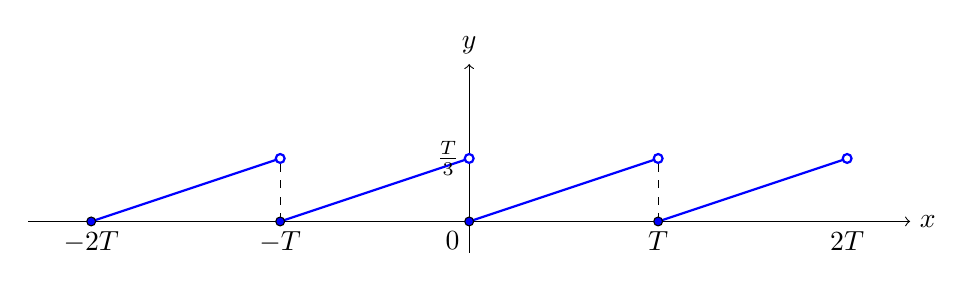
\begin{tikzpicture}[scale=0.8]
            \draw[->] (-7,0) -- (7,0) node[right] {$x$};
            \draw[->] (0,-0.5) -- (0,2.5) node[above] {$y$};

            \draw[dashed] (-3,0) -- (-3,1);
            \draw[dashed] (3,0) -- (3,1);

            \node[below left] at (0,0) {$0$};
            \node[below] at (3,0) {$T$};
            \node[below] at (-3,0) {$-T$};
            \node[below] at (6,0) {$2T$};
            \node[below] at (-6,0) {$-2T$};

            \draw[thick, blue] (-6, 0) -- (-3, 1);
            \draw[thick, blue] (-3, 0) -- (0, 1);
            \draw[thick, blue] (0, 0) -- (3, 1);
            \draw[thick, blue] (3, 0) -- (6, 1);

            \foreach \x in {-6, -3, 0, 3} {
                    \draw[fill=blue] (\x, 0) circle (2pt);
                }
            \foreach \x in {-3, 0, 3, 6} {
                    \draw[fill=white, draw=blue, thick] (\x, 1) circle (2pt);
                }
            \node[left] at (0,1) {$\frac{T}{3}$};
        \end{tikzpicture}
    \end{center}

    周期为 $T$，即 $2L = T \implies L = \frac{T}{2}$．计算 Fourier 系数：
    \begin{equation}
        a_0 = \frac{2}{T} \int_{0}^{T} \frac{x}{3} \d x = \frac{T}{3},
    \end{equation}

    \begin{equation}
        a_n = \frac{2}{T} \int_{0}^{T} \frac{x}{3} \cos \frac{2n\uppi x}{T} \d x = 0,
    \end{equation}

    \begin{equation}
        \begin{aligned}
            b_n & = \frac{2}{T} \int_{0}^{T} \frac{x}{3} \sin \frac{2n\uppi x}{T} \d x                                                                                              \\
                & = \frac{2}{3T} \left[ \left. -x \frac{T}{2n\uppi} \cos \frac{2n\uppi x}{T} \right|_{0}^{T} + \int_{0}^{T} \frac{T}{2n\uppi} \cos \frac{2n\uppi x}{T} \d x \right] \\
                & = -\frac{T}{3n\uppi}.
        \end{aligned}
    \end{equation}

    因此，函数的 Fourier 展开式为
    \begin{equation}
        \boxed{f(x) \sim \frac{T}{6} - \sum_{n=1}^{\infty} \frac{T}{3n\uppi} \sin \frac{2n\uppi x}{T}}.
    \end{equation}

    收敛情况：由于 $f(x)$ 周期延拓后分段光滑，当 $x \neq kT$ ($k \in \symbb{Z}$) 时，级数收敛于 $\frac{x}{3}$；当 $x = kT$ 时，级数收敛于 $\frac{T}{6}$．

    \ansitem{3}

    图形如下：
    \begin{center}
        \begin{tikzpicture}[scale=0.8]
            \draw[->] (-7,0) -- (7,0) node[right] {$x$};
            \draw[->] (0,-0.5) -- (0,3.5) node[above] {$y$};

            \draw[dashed] (-2,0) -- (-2,2.718);
            \draw[dashed] (2,0) -- (2,2.718);

            \node[below left] at (0,0) {$0$};
            \node[below] at (2,0) {$l$};
            \node[below] at (-2,0) {$-l$};
            \node[below] at (6,0) {$3l$};
            \node[below] at (-6,0) {$-3l$};

            \draw[thick, blue, domain=-2:2, samples=100] plot (\x, {exp(0.5*\x)});
            \draw[thick, blue, domain=2:6, samples=100] plot (\x, {exp(0.5*(\x-4))});
            \draw[thick, blue, domain=-6:-2, samples=100] plot (\x, {exp(0.5*(\x+4))});

            \foreach \x in {-6, -2, 2} {
                    \draw[fill=blue] (\x, 0.368) circle (2pt);
                }
            \foreach \x in {-2, 2, 6} {
                    \draw[fill=white, draw=blue, thick] (\x, 2.718) circle (2pt);
                }
            \node[left] at (0, 0.368) {$\e^{-al}$};
            \node[left] at (0, 2.718) {$\e^{al}$};
        \end{tikzpicture}
    \end{center}

    周期为 $2l$，即 $L = l$．计算 Fourier 系数：
    \begin{equation}
        a_0 = \frac{1}{l} \int_{-l}^{l} \e^{ax} \d x = \frac{2\sinh(al)}{al},
    \end{equation}

    \begin{equation}
        \begin{aligned}
            a_n & = \frac{1}{l} \int_{-l}^{l} \e^{ax} \cos \frac{n\uppi x}{l} \d x                                                                                                       \\
                & = \frac{1}{l} \left. \frac{\e^{ax} \left( a \cos \frac{n\uppi x}{l} + \frac{n\uppi}{l} \sin \frac{n\uppi x}{l} \right)}{a^2 + \frac{n^2\uppi^2}{l^2}} \right|_{-l}^{l} \\
                & = \frac{2al(-1)^n \sinh(al)}{a^2l^2 + n^2\uppi^2},
        \end{aligned}
    \end{equation}

    \begin{equation}
        \begin{aligned}
            b_n & = \frac{1}{l} \int_{-l}^{l} \e^{ax} \sin \frac{n\uppi x}{l} \d x                                                                                                       \\
                & = \frac{1}{l} \left. \frac{\e^{ax} \left( a \sin \frac{n\uppi x}{l} - \frac{n\uppi}{l} \cos \frac{n\uppi x}{l} \right)}{a^2 + \frac{n^2\uppi^2}{l^2}} \right|_{-l}^{l} \\
                & = \frac{2n\uppi(-1)^{n-1} \sinh(al)}{a^2l^2 + n^2\uppi^2}.
        \end{aligned}
    \end{equation}

    因此，函数的 Fourier 展开式为
    \begin{equation}
        \boxed{f(x) \sim \frac{\sinh(al)}{al} + \sum_{n=1}^{\infty} \frac{2\sinh(al)}{a^2l^2 + n^2\uppi^2} \left[ al(-1)^n \cos \frac{n\uppi x}{l} + n\uppi(-1)^{n-1} \sin \frac{n\uppi x}{l} \right]}.
    \end{equation}

    收敛情况：由于 $f(x)$ 周期延拓后分段光滑，当 $x \neq (2k+1)l$ ($k \in \symbb{Z}$) 时，级数收敛于 $\e^{ax}$；当 $x = (2k+1)l$ 时，级数收敛于 $\cosh(al)$．

    \ansitem{4}

    图形如下：
    \begin{center}
        \begin{tikzpicture}[scale=0.8]
            \draw[->] (-7,0) -- (7,0) node[right] {$x$};
            \draw[->] (0,-2) -- (0,2) node[above] {$y$};

            \node[below left] at (0,0) {$0$};
            \node[below] at (2,0) {$2$};
            \node[below] at (-2,0) {$-2$};
            \node[below] at (4,0) {$4$};
            \node[below] at (-4,0) {$-4$};

            \draw[thick, blue] (-6, -1) -- (-5, -1);
            \draw[thick, blue] (-5, 1) -- (-3, 1);
            \draw[thick, blue] (-3, -1) -- (-1, -1);
            \draw[thick, blue] (-1, 1) -- (1, 1);
            \draw[thick, blue] (1, -1) -- (3, -1);
            \draw[thick, blue] (3, 1) -- (5, 1);
            \draw[thick, blue] (5, -1) -- (6, -1);

            \foreach \x in {-5, -3, -1, 1, 3, 5} {
                    \draw[fill=white, draw=blue, thick] (\x, 1) circle (2pt);
                }
            \foreach \x in {-6, -5, -3, -1, 1, 3, 5, 6} {
                    \draw[fill=blue] (\x, -1) circle (2pt);
                }
            \node[left] at (0, 1) {$1$};
            \node[left] at (0, -1) {$-1$};
        \end{tikzpicture}
    \end{center}

    周期为 $4$，即 $2L = 4 \implies L = 2$．因为 $f(x)$ 是偶函数，所以 $b_n = 0$．
    \begin{equation}
        a_0 = \frac{2}{2} \int_{0}^{2} f(x) \d x = \int_{0}^{1} 1 \d x + \int_{1}^{2} (-1) \d x = 0,
    \end{equation}

    \begin{equation}
        \begin{aligned}
            a_n & = \frac{2}{2} \int_{0}^{2} f(x) \cos \frac{n\uppi x}{2} \d x                            \\
                & = \int_{0}^{1} \cos \frac{n\uppi x}{2} \d x - \int_{1}^{2} \cos \frac{n\uppi x}{2} \d x \\
                & = \frac{4}{n\uppi} \sin \frac{n\uppi}{2}.
        \end{aligned}
    \end{equation}

    当 $n = 2k$ ($k \in \symbb{N}^*$) 时，$a_{2k} = 0$；当 $n = 2k-1$ ($k \in \symbb{N}^*$) 时，$a_{2k-1} = \frac{4(-1)^{k-1}}{(2k-1)\uppi}$．

    因此，函数的 Fourier 展开式为
    \begin{equation}
        \boxed{f(x) \sim \sum_{k=1}^{\infty} \frac{4(-1)^{k-1}}{(2k-1)\uppi} \cos \frac{(2k-1)\uppi x}{2}}.
    \end{equation}

    收敛情况：由于 $f(x)$ 周期延拓后分段光滑，当 $x \neq 2k+1$ ($k \in \symbb{Z}$) 时，级数收敛于 $f(x)$；当 $x = 2k+1$ 时，级数收敛于 $0$．
\end{solution}

\begin{problem}{正弦与余弦级数展开}{Sine-Cosine-Fourier-Expansion}
    把下列函数展开成正弦级数和余弦级数：
    \begin{enumerate}
        \item $f(x) = 2x^2 \quad (0 \leqslant x \leqslant \uppi)$;
        \item $f(x) = \begin{dcases} A, & 0 \leqslant x < \frac{l}{2}, \\ 0, & \frac{l}{2} \leqslant x \leqslant l; \end{dcases}$
        \item $f(x) = \begin{dcases} 1 - \frac{x}{2h}, & 0 \leqslant x \leqslant 2h, \\ 0, & 2h < x \leqslant \uppi. \end{dcases}$
    \end{enumerate}
\end{problem}

\begin{solution}
    \ansitem{1}
    对于函数 $f(x) = 2x^2$ ($0 \leqslant x \leqslant \uppi$)，其奇延拓与偶延拓的图形如下．

    \begin{center}
        \begin{tikzpicture}[scale=0.55]
            \draw[->] (-7,0) -- (7,0) node[right] {$x$};
            \draw[->] (0,-2.5) -- (0,2.5) node[above] {$y$};
            \node[below left] at (0,0) {$0$};
            \node[below] at (3.1416,0) {$\uppi$};
            \node[below] at (-3.1416,0) {$-\uppi$};
            \node[below] at (6.2832,0) {$2\uppi$};
            \node[below] at (-6.2832,0) {$-2\uppi$};

            \draw[thick, blue, domain=-6.2832:-3.1416, samples=100] plot (\x, {2*((\x+6.2832)/3.1416)^2});
            \draw[thick, blue, domain=-3.1416:0, samples=100] plot (\x, {-2*(\x/3.1416)^2});
            \draw[thick, blue, domain=0:3.1416, samples=100] plot (\x, {2*(\x/3.1416)^2});
            \draw[thick, blue, domain=3.1416:6.2832, samples=100] plot (\x, {-2*((\x-6.2832)/3.1416)^2});

            \draw[fill=blue] (0,0) circle (2pt);
            \draw[fill=blue] (6.2832,0) circle (2pt);
            \draw[fill=blue] (-6.2832,0) circle (2pt);
            \draw[fill=white, draw=blue, thick] (3.1416,2) circle (2pt);
            \draw[fill=white, draw=blue, thick] (3.1416,-2) circle (2pt);
            \draw[fill=blue] (3.1416,0) circle (2pt);
            \draw[fill=white, draw=blue, thick] (-3.1416,2) circle (2pt);
            \draw[fill=white, draw=blue, thick] (-3.1416,-2) circle (2pt);
            \draw[fill=blue] (-3.1416,0) circle (2pt);
        \end{tikzpicture}
        \qquad
        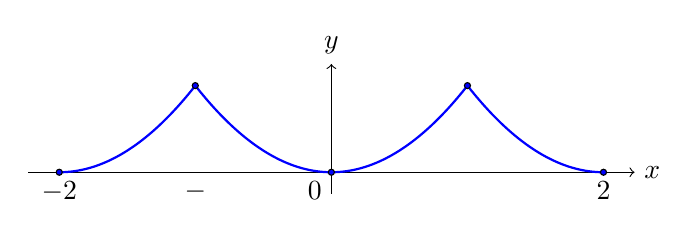
\begin{tikzpicture}[scale=0.55]
            \draw[->] (-7,0) -- (7,0) node[right] {$x$};
            \draw[->] (0,-0.5) -- (0,2.5) node[above] {$y$};
            \node[below left] at (0,0) {$0$};
            \node[below] at (3.1416,0) {$\uppi$};
            \node[below] at (-3.1416,0) {$-\uppi$};
            \node[below] at (6.2832,0) {$2\uppi$};
            \node[below] at (-6.2832,0) {$-2\uppi$};

            \draw[thick, blue, domain=-6.2832:-3.1416, samples=100] plot (\x, {2*((\x+6.2832)/3.1416)^2});
            \draw[thick, blue, domain=-3.1416:3.1416, samples=100] plot (\x, {2*(\x/3.1416)^2});
            \draw[thick, blue, domain=3.1416:6.2832, samples=100] plot (\x, {2*((\x-6.2832)/3.1416)^2});

            \draw[fill=blue] (0,0) circle (2pt);
            \draw[fill=blue] (3.1416,2) circle (2pt);
            \draw[fill=blue] (-3.1416,2) circle (2pt);
            \draw[fill=blue] (6.2832,0) circle (2pt);
            \draw[fill=blue] (-6.2832,0) circle (2pt);
        \end{tikzpicture}
        \\
        \small 左：奇延拓（正弦级数） \qquad\qquad 右：偶延拓（余弦级数）
    \end{center}

    计算正弦级数的系数：
    \begin{equation}
        \begin{aligned}
            b_n & = \frac{2}{\uppi} \int_{0}^{\uppi} 2x^2 \sin(nx) \d x                                                                                                                                 \\
                & = \frac{4}{\uppi} \left[ \left. -x^2 \frac{\cos(nx)}{n} \right|_{0}^{\uppi} + \int_{0}^{\uppi} \frac{2x \cos(nx)}{n} \d x \right]                                                     \\
                & = \frac{4}{\uppi} \left[ \frac{\uppi^2 (-1)^{n-1}}{n} + \frac{2}{n} \left( \left. \frac{x \sin(nx)}{n} \right|_{0}^{\uppi} - \int_{0}^{\uppi} \frac{\sin(nx)}{n} \d x \right) \right] \\
                & = \frac{4\uppi (-1)^{n-1}}{n} - \frac{8(1 - (-1)^n)}{\uppi n^3}.
        \end{aligned}
    \end{equation}

    计算余弦级数的系数：
    \begin{equation}
        a_0 = \frac{2}{\uppi} \int_{0}^{\uppi} 2x^2 \d x = \frac{4\uppi^2}{3},
    \end{equation}
    \begin{equation}
        \begin{aligned}
            a_n & = \frac{2}{\uppi} \int_{0}^{\uppi} 2x^2 \cos(nx) \d x                                                                            \\
                & = \frac{4}{\uppi} \left[ \left. x^2 \frac{\sin(nx)}{n} \right|_{0}^{\uppi} - \int_{0}^{\uppi} \frac{2x \sin(nx)}{n} \d x \right] \\
                & = -\frac{8}{\uppi n} \left[ \left. -x \frac{\cos(nx)}{n} \right|_{0}^{\uppi} + \int_{0}^{\uppi} \frac{\cos(nx)}{n} \d x \right]  \\
                & = \frac{8 (-1)^n}{n^2}.
        \end{aligned}
    \end{equation}

    因此，展开为正弦级数为
    \begin{equation}
        \boxed{f(x) \sim \sum_{n=1}^{\infty} \left[ \frac{4\uppi(-1)^{n-1}}{n} - \frac{8(1 - (-1)^n)}{\uppi n^3} \right] \sin(nx)},
    \end{equation}
    展开为余弦级数为
    \begin{equation}
        \boxed{f(x) \sim \frac{2\uppi^2}{3} + \sum_{n=1}^{\infty} \frac{8(-1)^n}{n^2} \cos(nx)}.
    \end{equation}

    收敛情况：对于正弦级数，当 $x \in (2k\uppi, (2k+1)\uppi)$ 时收敛于 $2(x-2k\uppi)^2$，当 $x \in ((2k-1)\uppi, 2k\uppi)$ 时收敛于 $-2(x-2k\uppi)^2$，当 $x = k\uppi$ 时收敛于 $0$；对于余弦级数，在整个实数轴上均收敛于其连续的偶周期延拓函数．

    \ansitem{2}
    对于函数 $f(x)$，其奇延拓与偶延拓图形如下．

    \begin{center}
        \begin{tikzpicture}[scale=0.75]
            \draw[->] (-5,0) -- (5,0) node[right] {$x$};
            \draw[->] (0,-2) -- (0,2) node[above] {$y$};
            \node[below left] at (0,0) {$0$};
            \node[below] at (2,0) {$l$};
            \node[below] at (-2,0) {$-l$};
            \node[below] at (4,0) {$2l$};
            \node[below] at (-4,0) {$-2l$};
            \node[below] at (1,0) {$\frac{l}{2}$};
            \node[below] at (-1,0) {$-\frac{l}{2}$};

            \draw[thick, blue] (-2, 0) -- (-1, 0);
            \draw[thick, blue] (-1, -1.5) -- (0, -1.5);
            \draw[thick, blue] (0, 1.5) -- (1, 1.5);
            \draw[thick, blue] (1, 0) -- (2, 0);
            \draw[thick, blue] (2, 0) -- (3, 0);
            \draw[thick, blue] (3, -1.5) -- (4, -1.5);
            \draw[thick, blue] (-3, 0) -- (-2, 0);
            \draw[thick, blue] (-4, 1.5) -- (-3, 1.5);

            \draw[fill=white, draw=blue, thick] (0, 1.5) circle (2pt);
            \draw[fill=white, draw=blue, thick] (0, -1.5) circle (2pt);
            \draw[fill=blue] (0,0) circle (2pt);
            \draw[fill=white, draw=blue, thick] (1, 1.5) circle (2pt);
            \draw[fill=white, draw=blue, thick] (1, 0) circle (2pt);
            \draw[fill=blue] (1, 0.75) circle (2pt);
            \draw[fill=white, draw=blue, thick] (-1, -1.5) circle (2pt);
            \draw[fill=white, draw=blue, thick] (-1, 0) circle (2pt);
            \draw[fill=blue] (-1, -0.75) circle (2pt);
            \draw[fill=blue] (2, 0) circle (2pt);
            \draw[fill=blue] (-2, 0) circle (2pt);
            \draw[fill=white, draw=blue, thick] (3, 0) circle (2pt);
            \draw[fill=white, draw=blue, thick] (3, -1.5) circle (2pt);
            \draw[fill=blue] (3, -0.75) circle (2pt);
            \draw[fill=white, draw=blue, thick] (-3, 0) circle (2pt);
            \draw[fill=white, draw=blue, thick] (-3, 1.5) circle (2pt);
            \draw[fill=blue] (-3, 0.75) circle (2pt);

            \node[left] at (0, 1.5) {$A$};
            \node[left] at (0, -1.5) {$-A$};
        \end{tikzpicture}
        \qquad
        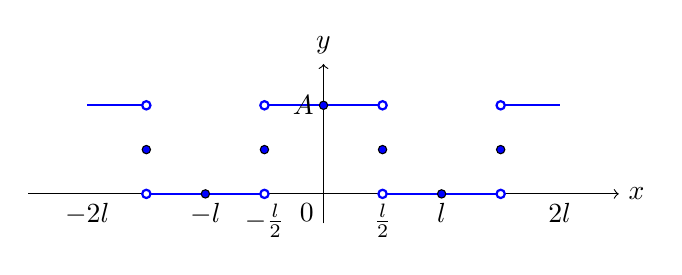
\begin{tikzpicture}[scale=0.75]
            \draw[->] (-5,0) -- (5,0) node[right] {$x$};
            \draw[->] (0,-0.5) -- (0,2.2) node[above] {$y$};
            \node[below left] at (0,0) {$0$};
            \node[below] at (2,0) {$l$};
            \node[below] at (-2,0) {$-l$};
            \node[below] at (4,0) {$2l$};
            \node[below] at (-4,0) {$-2l$};
            \node[below] at (1,0) {$\frac{l}{2}$};
            \node[below] at (-1,0) {$-\frac{l}{2}$};

            \draw[thick, blue] (-2, 0) -- (-1, 0);
            \draw[thick, blue] (-1, 1.5) -- (1, 1.5);
            \draw[thick, blue] (1, 0) -- (2, 0);
            \draw[thick, blue] (2, 0) -- (3, 0);
            \draw[thick, blue] (3, 1.5) -- (4, 1.5);
            \draw[thick, blue] (-3, 0) -- (-2, 0);
            \draw[thick, blue] (-4, 1.5) -- (-3, 1.5);

            \draw[fill=white, draw=blue, thick] (1, 1.5) circle (2pt);
            \draw[fill=white, draw=blue, thick] (1, 0) circle (2pt);
            \draw[fill=blue] (1, 0.75) circle (2pt);
            \draw[fill=white, draw=blue, thick] (-1, 1.5) circle (2pt);
            \draw[fill=white, draw=blue, thick] (-1, 0) circle (2pt);
            \draw[fill=blue] (-1, 0.75) circle (2pt);
            \draw[fill=blue] (0, 1.5) circle (2pt);
            \draw[fill=blue] (2, 0) circle (2pt);
            \draw[fill=blue] (-2, 0) circle (2pt);
            \draw[fill=white, draw=blue, thick] (3, 0) circle (2pt);
            \draw[fill=white, draw=blue, thick] (3, 1.5) circle (2pt);
            \draw[fill=blue] (3, 0.75) circle (2pt);
            \draw[fill=white, draw=blue, thick] (-3, 0) circle (2pt);
            \draw[fill=white, draw=blue, thick] (-3, 1.5) circle (2pt);
            \draw[fill=blue] (-3, 0.75) circle (2pt);

            \node[left] at (0, 1.5) {$A$};
        \end{tikzpicture}
        \\
        \small 左：奇延拓（正弦级数） \qquad\qquad 右：偶延拓（余弦级数）
    \end{center}

    计算正弦级数的系数：
    \begin{equation}
        b_n = \frac{2}{l} \int_{0}^{\frac{l}{2}} A \sin \frac{n\uppi x}{l} \d x = \frac{2A}{n\uppi} \left( 1 - \cos \frac{n\uppi}{2} \right).
    \end{equation}

    计算余弦级数的系数：
    \begin{equation}
        a_0 = \frac{2}{l} \int_{0}^{\frac{l}{2}} A \d x = A,
    \end{equation}
    \begin{equation}
        a_n = \frac{2}{l} \int_{0}^{\frac{l}{2}} A \cos \frac{n\uppi x}{l} \d x = \frac{2A}{n\uppi} \sin \frac{n\uppi}{2}.
    \end{equation}

    因此，展开为正弦级数为
    \begin{equation}
        \boxed{f(x) \sim \sum_{n=1}^{\infty} \frac{2A}{n\uppi} \left( 1 - \cos \frac{n\uppi}{2} \right) \sin \frac{n\uppi x}{l}},
    \end{equation}
    展开为余弦级数为
    \begin{equation}
        \boxed{f(x) \sim \frac{A}{2} + \sum_{n=1}^{\infty} \frac{2A}{n\uppi} \sin \frac{n\uppi}{2} \cos \frac{n\uppi x}{l}}.
    \end{equation}

    收敛情况：当 $x \neq kl \pm \frac{l}{2}$ 且 $x \neq kl$ 时，两级数均收敛于对应延拓函数值．在间断点处，正弦级数在 $x = kl \pm \frac{l}{2}$ 时收敛于 $\pm \frac{A}{2}$，在 $x = kl$ 时收敛于 $0$；余弦级数在 $x = kl \pm \frac{l}{2}$ 时收敛于 $\frac{A}{2}$．

    \ansitem{3}
    对于函数 $f(x)$，其奇延拓与偶延拓图形如下．

    \begin{center}
        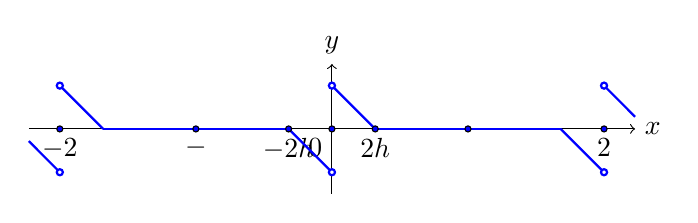
\begin{tikzpicture}[scale=0.55]
            \draw[->] (-7,0) -- (7,0) node[right] {$x$};
            \draw[->] (0,-1.5) -- (0,1.5) node[above] {$y$};
            \node[below left] at (0,0) {$0$};
            \node[below] at (3.1416,0) {$\uppi$};
            \node[below] at (-3.1416,0) {$-\uppi$};
            \node[below] at (6.2832,0) {$2\uppi$};
            \node[below] at (-6.2832,0) {$-2\uppi$};
            \node[below] at (1,0) {$2h$};
            \node[below] at (-1,0) {$-2h$};

            \draw[thick, blue] (-3.1416, 0) -- (-1, 0);
            \draw[thick, blue] (-1, 0) -- (0, -1);
            \draw[thick, blue] (0, 1) -- (1, 0);
            \draw[thick, blue] (1, 0) -- (3.1416, 0);
            \draw[thick, blue] (3.1416, 0) -- (5.2832, 0);
            \draw[thick, blue] (5.2832, 0) -- (6.2832, -1);
            \draw[thick, blue] (6.2832, 1) -- (7, 0.28);
            \draw[thick, blue] (-7, -0.28) -- (-6.2832, -1);
            \draw[thick, blue] (-6.2832, 1) -- (-5.2832, 0);
            \draw[thick, blue] (-5.2832, 0) -- (-3.1416, 0);

            \draw[fill=white, draw=blue, thick] (0, 1) circle (2pt);
            \draw[fill=white, draw=blue, thick] (0, -1) circle (2pt);
            \draw[fill=blue] (0,0) circle (2pt);
            \draw[fill=white, draw=blue, thick] (6.2832, 1) circle (2pt);
            \draw[fill=white, draw=blue, thick] (6.2832, -1) circle (2pt);
            \draw[fill=blue] (6.2832, 0) circle (2pt);
            \draw[fill=white, draw=blue, thick] (-6.2832, 1) circle (2pt);
            \draw[fill=white, draw=blue, thick] (-6.2832, -1) circle (2pt);
            \draw[fill=blue] (-6.2832, 0) circle (2pt);
            \draw[fill=blue] (1,0) circle (2pt);
            \draw[fill=blue] (-1,0) circle (2pt);
            \draw[fill=blue] (3.1416,0) circle (2pt);
            \draw[fill=blue] (-3.1416,0) circle (2pt);
        \end{tikzpicture}
        \qquad
        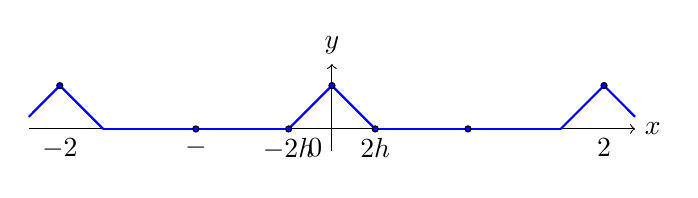
\begin{tikzpicture}[scale=0.55]
            \draw[->] (-7,0) -- (7,0) node[right] {$x$};
            \draw[->] (0,-0.5) -- (0,1.5) node[above] {$y$};
            \node[below left] at (0,0) {$0$};
            \node[below] at (3.1416,0) {$\uppi$};
            \node[below] at (-3.1416,0) {$-\uppi$};
            \node[below] at (6.2832,0) {$2\uppi$};
            \node[below] at (-6.2832,0) {$-2\uppi$};
            \node[below] at (1,0) {$2h$};
            \node[below] at (-1,0) {$-2h$};

            \draw[thick, blue] (-3.1416, 0) -- (-1, 0);
            \draw[thick, blue] (-1, 0) -- (0, 1);
            \draw[thick, blue] (0, 1) -- (1, 0);
            \draw[thick, blue] (1, 0) -- (3.1416, 0);
            \draw[thick, blue] (3.1416, 0) -- (5.2832, 0);
            \draw[thick, blue] (5.2832, 0) -- (6.2832, 1);
            \draw[thick, blue] (6.2832, 1) -- (7, 0.28);
            \draw[thick, blue] (-7, 0.28) -- (-6.2832, 1);
            \draw[thick, blue] (-6.2832, 1) -- (-5.2832, 0);
            \draw[thick, blue] (-5.2832, 0) -- (-3.1416, 0);

            \draw[fill=blue] (0, 1) circle (2pt);
            \draw[fill=blue] (6.2832, 1) circle (2pt);
            \draw[fill=blue] (-6.2832, 1) circle (2pt);
            \draw[fill=blue] (1, 0) circle (2pt);
            \draw[fill=blue] (-1, 0) circle (2pt);
            \draw[fill=blue] (3.1416, 0) circle (2pt);
            \draw[fill=blue] (-3.1416, 0) circle (2pt);
        \end{tikzpicture}
        \\
        \small 左：奇延拓（正弦级数） \qquad\qquad 右：偶延拓（余弦级数）
    \end{center}

    计算正弦级数的系数：
    \begin{equation}
        \begin{aligned}
            b_n & = \frac{2}{\uppi} \int_{0}^{2h} \left( 1 - \frac{x}{2h} \right) \sin(nx) \d x                                                                          \\
                & = \frac{2}{\uppi} \left[ \left. -\left( 1 - \frac{x}{2h} \right) \frac{\cos(nx)}{n} \right|_{0}^{2h} - \int_{0}^{2h} \frac{\cos(nx)}{2hn} \d x \right] \\
                & = \frac{2}{n\uppi} - \frac{\sin(2nh)}{hn^2\uppi}.
        \end{aligned}
    \end{equation}

    计算余弦级数的系数：
    \begin{equation}
        a_0 = \frac{2}{\uppi} \int_{0}^{2h} \left( 1 - \frac{x}{2h} \right) \d x = \frac{2h}{\uppi},
    \end{equation}
    \begin{equation}
        \begin{aligned}
            a_n & = \frac{2}{\uppi} \int_{0}^{2h} \left( 1 - \frac{x}{2h} \right) \cos(nx) \d x                                                                         \\
                & = \frac{2}{\uppi} \left[ \left. \left( 1 - \frac{x}{2h} \right) \frac{\sin(nx)}{n} \right|_{0}^{2h} + \int_{0}^{2h} \frac{\sin(nx)}{2hn} \d x \right] \\
                & = \frac{1 - \cos(2nh)}{hn^2\uppi} = \frac{2\sin^2(nh)}{hn^2\uppi}.
        \end{aligned}
    \end{equation}

    因此，展开为正弦级数为
    \begin{equation}
        \boxed{f(x) \sim \sum_{n=1}^{\infty} \left[ \frac{2}{n\uppi} - \frac{\sin(2nh)}{hn^2\uppi} \right] \sin(nx)},
    \end{equation}
    展开为余弦级数为
    \begin{equation}
        \boxed{f(x) \sim \frac{h}{\uppi} + \sum_{n=1}^{\infty} \frac{2\sin^2(nh)}{hn^2\uppi} \cos(nx)}.
    \end{equation}

    收敛情况：由于 $f(x)$ 连续，其偶延拓在整个实数轴上均连续，故余弦级数在整个实数轴上都收敛于该偶周期延拓函数；而正弦级数在其奇延拓的间断点 $x = 2k\uppi$ ($k \in \symbb{Z}$) 处收敛于 $0$，在其他点处均收敛于对应奇周期延拓函数值．
\end{solution}

\begin{problem}{确定Fourier系数中的常数}{Fourier-Coefficient-Constant}
    已知函数的 Fourier 级数展开式，求常数 $a$ 的值．
    \begin{enumerate}
        \item $\sum_{n=1}^{\infty} \frac{\cos(2n-1)x}{(2n-1)^2} = a(2a - |x|)$，其中 $-\uppi \leqslant x \leqslant \uppi$;
        \item $\sum_{n=1}^{\infty} \frac{(-1)^{n-1}}{n} \sin nx = ax$，其中 $-\uppi < x < \uppi$．
    \end{enumerate}
\end{problem}

\begin{solution}
    \ansitem{1} $a = \frac{\uppi}{4}$．

    图形如下：
    \begin{center}
        \begin{tikzpicture}[scale=0.8]
            \draw[->] (-7,0) -- (7,0) node[right] {$x$};
            \draw[->] (0,-2.5) -- (0,2.5) node[above] {$y$};

            \draw[dashed] (-3.1416,-2) -- (-3.1416,2);
            \draw[dashed] (3.1416,-2) -- (3.1416,2);

            \node[below left] at (0,0) {$0$};
            \node[below] at (3.1416,0) {$\uppi$};
            \node[below] at (-3.1416,0) {$-\uppi$};
            \node[below] at (6.2832,0) {$2\uppi$};
            \node[below] at (-6.2832,0) {$-2\uppi$};

            % 绘制三角波
            \draw[thick, blue] (-6.2832, 1.2337) -- (-3.1416, -1.2337) -- (0, 1.2337) -- (3.1416, -1.2337) -- (6.2832, 1.2337);

            \draw[dashed] (-6.5, 1.2337) -- (6.5, 1.2337);
            \draw[dashed] (-6.5, -1.2337) -- (6.5, -1.2337);
            \node[left] at (0, 1.2337) {$\frac{\uppi^2}{8}$};
            \node[left] at (0, -1.2337) {$-\frac{\uppi^2}{8}$};

            \draw[fill=blue] (0, 1.2337) circle (2pt);
            \draw[fill=blue] (3.1416, -1.2337) circle (2pt);
            \draw[fill=blue] (-3.1416, -1.2337) circle (2pt);
            \draw[fill=blue] (6.2832, 1.2337) circle (2pt);
            \draw[fill=blue] (-6.2832, 1.2337) circle (2pt);
        \end{tikzpicture}
    \end{center}

    令 $f(x) = a(2a - |x|)$．由于给定的 Fourier 级数不含常数项（即 $a_0 = 0$），因此必须有
    \begin{equation}
        a_0 = \frac{1}{\uppi} \int_{-\uppi}^{\uppi} a(2a - |x|) \d x = 0.
    \end{equation}
    假定 $a \neq 0$，则有
    \begin{equation}
        \int_{0}^{\uppi} (2a - x) \d x = \left[ 2ax - \frac{x^2}{2} \right]_{0}^{\uppi} = 2a\uppi - \frac{\uppi^2}{2} = 0,
    \end{equation}
    解得
    \begin{equation}
        a = \frac{\uppi}{4}.
    \end{equation}
    此时 $f(x) = \frac{\uppi}{4} \left( \frac{\uppi}{2} - |x| \right)$．验证其 Fourier 余弦系数：
    \begin{equation}
        \begin{aligned}
            a_n & = \frac{2}{\uppi} \int_{0}^{\uppi} \frac{\uppi}{4} \left( \frac{\uppi}{2} - x \right) \cos(nx) \d x                                                      \\
                & = \frac{1}{2} \left[ \left. \left( \frac{\uppi}{2} - x \right) \frac{\sin(nx)}{n} \right|_{0}^{\uppi} + \int_{0}^{\uppi} \frac{\sin(nx)}{n} \d x \right] \\
                & = \frac{1 - (-1)^n}{2n^2}.
        \end{aligned}
    \end{equation}
    当 $n = 2k$ 时，$a_{2k} = 0$；当 $n = 2k-1$ 时，$a_{2k-1} = \frac{1}{(2k-1)^2}$．系数与原级数完全相符．
    因此，常数 $a$ 的值为
    \begin{equation}
        \boxed{a = \frac{\uppi}{4}}.
    \end{equation}

    \ansitem{2} $a = \frac{1}{2}$．

    图形如下：
    \begin{center}
        \begin{tikzpicture}[scale=0.8]
            \draw[->] (-7,0) -- (7,0) node[right] {$x$};
            \draw[->] (0,-2.5) -- (0,2.5) node[above] {$y$};

            \draw[dashed] (-3.1416,-2) -- (-3.1416,2);
            \draw[dashed] (3.1416,-2) -- (3.1416,2);

            \node[below left] at (0,0) {$0$};
            \node[below] at (3.1416,0) {$\uppi$};
            \node[below] at (-3.1416,0) {$-\uppi$};
            \node[below] at (6.2832,0) {$2\uppi$};
            \node[below] at (-6.2832,0) {$-2\uppi$};

            % 绘制周期锯齿波
            \draw[thick, blue] (-3.1416, -1.5708) -- (3.1416, 1.5708);
            \draw[thick, blue] (3.1416, -1.5708) -- (6.2832, 0) -- (7, 0.3584);
            \draw[thick, blue] (-7, -0.3584) -- (-6.2832, 0) -- (-3.1416, 1.5708);

            % 间断点处的空心与实心圆点
            \foreach \x in {-3.1416, 3.1416} {
                    \draw[fill=white, draw=blue, thick] (\x, 1.5708) circle (2pt);
                    \draw[fill=white, draw=blue, thick] (\x, -1.5708) circle (2pt);
                    \draw[fill=blue] (\x, 0) circle (2pt);
                }
            \draw[fill=blue] (0, 0) circle (2pt);
            \draw[fill=blue] (6.2832, 0) circle (2pt);
            \draw[fill=blue] (-6.2832, 0) circle (2pt);

            \draw[dashed] (-3.5, 1.5708) -- (3.5, 1.5708);
            \draw[dashed] (-3.5, -1.5708) -- (3.5, -1.5708);
            \node[left] at (0, 1.5708) {$\frac{\uppi}{2}$};
            \node[left] at (0, -1.5708) {$-\frac{\uppi}{2}$};
        \end{tikzpicture}
    \end{center}

    令 $f(x) = ax$．由于 $f(x)$ 是在 $(-\uppi, \uppi)$ 上的奇函数，其 Fourier 展开式只包含正弦项，系数 $b_n$ 为
    \begin{equation}
        \begin{aligned}
            b_n & = \frac{2}{\uppi} \int_{0}^{\uppi} ax \sin(nx) \d x                                                                           \\
                & = \frac{2a}{\uppi} \left[ \left. -x \frac{\cos(nx)}{n} \right|_{0}^{\uppi} + \int_{0}^{\uppi} \frac{\cos(nx)}{n} \d x \right] \\
                & = \frac{2a}{\uppi} \left[ -\frac{\uppi (-1)^n}{n} \right]                                                                     \\
                & = \frac{2a (-1)^{n-1}}{n}.
        \end{aligned}
    \end{equation}
    与已知的 Fourier 级数展开式系数对比，可得
    \begin{equation}
        \frac{2a (-1)^{n-1}}{n} = \frac{(-1)^{n-1}}{n},
    \end{equation}
    从而解得
    \begin{equation}
        \boxed{a = \frac{1}{2}}.
    \end{equation}
\end{solution}

\begin{problem}{Fourier级数和函数}{Fourier-Series-Sum-Function}
    \begin{enumerate}
        \item 设
              \begin{equation}
                  f(x) = \begin{dcases} x, & 0 \leqslant x \leqslant \frac{1}{2}, \\ 2 - 2x, & \frac{1}{2} < x < 1, \end{dcases}
              \end{equation}
              \begin{equation}
                  S(x) = \frac{a_0}{2} + \sum_{n=1}^{\infty} a_n \cos n \uppi x, \quad -\infty < x < +\infty
              \end{equation}
              其中 $a_n = 2 \int_{0}^{1} f(x) \cos n \uppi x \d x \ (n = 0, 1, 2, \cdots)$．求 $S\left(\frac{9}{4}\right)$、$S\left(-\frac{5}{2}\right)$；
        \item 设
              \begin{equation}
                  f(x) = \begin{dcases} -1, & -\uppi < x \leqslant 0, \\ 1 + x^2, & 0 < x \leqslant \uppi, \end{dcases}
              \end{equation}
              则其以 $2\uppi$ 为周期的 Fourier 级数的和函数为 $S(x), -\infty < x < +\infty$．求 $S(3\uppi)$、$S(-4\uppi)$．
    \end{enumerate}
\end{problem}

\begin{solution}
    \ansitem{1}

    对小问 (1)，$S(x)$ 为 $f(x)$ 的偶周期延拓（周期 $T = 2$）的 Fourier 级数和函数．其图形如下：
    \begin{center}
        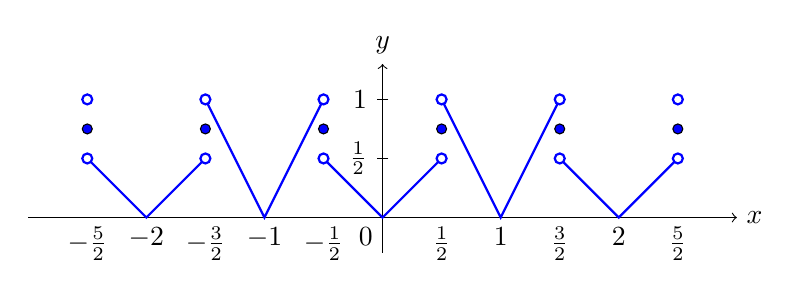
\begin{tikzpicture}[scale=1.5]
            \draw[->] (-3,0) -- (3,0) node[right] {$x$};
            \draw[->] (0,-0.3) -- (0,1.3) node[above] {$y$};

            \node[below left] at (0,0) {$0$};
            \node[below] at (0.5,0) {$\frac{1}{2}$};
            \node[below] at (1,0) {$1$};
            \node[below] at (1.5,0) {$\frac{3}{2}$};
            \node[below] at (2,0) {$2$};
            \node[below] at (2.5,0) {$\frac{5}{2}$};
            \node[below] at (-0.5,0) {$-\frac{1}{2}$};
            \node[below] at (-1,0) {$-1$};
            \node[below] at (-1.5,0) {$-\frac{3}{2}$};
            \node[below] at (-2,0) {$-2$};
            \node[below] at (-2.5,0) {$-\frac{5}{2}$};

            \draw (0.05,0.5) -- (-0.05,0.5) node[left] {$\frac{1}{2}$};
            \draw (0.05,1) -- (-0.05,1) node[left] {$1$};

            \draw[thick, blue] (-2.5, 0.5) -- (-2, 0) -- (-1.5, 0.5);
            \draw[thick, blue] (-1.5, 1) -- (-1, 0) -- (-0.5, 1);
            \draw[thick, blue] (-0.5, 0.5) -- (0, 0) -- (0.5, 0.5);
            \draw[thick, blue] (0.5, 1) -- (1, 0) -- (1.5, 1);
            \draw[thick, blue] (1.5, 0.5) -- (2, 0) -- (2.5, 0.5);

            \foreach \x in {-2.5, -0.5, 1.5} {
                    \draw[fill=white, draw=blue, thick] (\x, 0.5) circle (1.2pt);
                    \draw[fill=white, draw=blue, thick] (\x, 1) circle (1.2pt);
                    \draw[fill=blue] (\x, 0.75) circle (1.2pt);
                }
            \foreach \x in {-1.5, 0.5, 2.5} {
                    \draw[fill=white, draw=blue, thick] (\x, 0.5) circle (1.2pt);
                    \draw[fill=white, draw=blue, thick] (\x, 1) circle (1.2pt);
                    \draw[fill=blue] (\x, 0.75) circle (1.2pt);
                }
        \end{tikzpicture}
    \end{center}

    由 Dirichlet 收敛定理，在连续点处 $S(x) = f(x)$，在跳跃间断点 $x_0$ 处 $S(x_0) = \frac{f(x_0^-) + f(x_0^+)}{2}$．
    因为 $T = 2$，有：
    \begin{equation}
        S\left(\frac{9}{4}\right) = S\left(\frac{9}{4} - 2\right) = S\left(\frac{1}{4}\right).
    \end{equation}
    由于 $x = \frac{1}{4}$ 为连续点，故有：
    \begin{equation}
        S\left(\frac{1}{4}\right) = f\left(\frac{1}{4}\right) = \frac{1}{4}.
    \end{equation}
    同理：
    \begin{equation}
        S\left(-\frac{5}{2}\right) = S\left(-\frac{5}{2} + 2\right) = S\left(-\frac{1}{2}\right) = S\left(\frac{1}{2}\right).
    \end{equation}
    因为 $x = \frac{1}{2}$ 是跳跃间断点，其左右极限为：
    \begin{equation}
        f\left(\frac{1}{2}^-\right) = \frac{1}{2}, \quad f\left(\frac{1}{2}^+\right) = 2 - 2\left(\frac{1}{2}\right) = 1.
    \end{equation}
    故有：
    \begin{equation}
        S\left(\frac{1}{2}\right) = \frac{\frac{1}{2} + 1}{2} = \frac{3}{4}.
    \end{equation}

    因此，最终结果为：
    \begin{equation}
        \boxed{S\left(\frac{9}{4}\right) = \frac{1}{4}, \quad S\left(-\frac{5}{2}\right) = \frac{3}{4}}.
    \end{equation}

    \ansitem{2}

    对小问 (2)，$S(x)$ 是 $f(x)$ 周期延拓（周期 $T = 2\uppi$）的 Fourier 级数和函数．其图形如下：
    \begin{center}
        \begin{tikzpicture}[scale=0.8]
            \draw[->] (-8,0) -- (8,0) node[right] {$x$};
            \draw[->] (0,-2) -- (0,12) node[above] {$y$};

            \node[below left] at (0,0) {$0$};
            \node[below] at (3.1416,0) {$\uppi$};
            \node[below] at (6.2832,0) {$2\uppi$};
            \node[below] at (-3.1416,0) {$-\uppi$};
            \node[below] at (-6.2832,0) {$-2\uppi$};

            \draw (-0.1, -1) -- (0.1, -1) node[right] {$-1$};
            \draw (-0.1, 1) -- (0.1, 1) node[left] {$1$};
            \draw (-0.1, 10.87) -- (0.1, 10.87) node[left] {$1+\uppi^2$};
            \draw (-0.1, 4.93) -- (0.1, 4.93) node[left] {$\frac{\uppi^2}{2}$};

            \draw[thick, blue] (-3.1416, -1) -- (0, -1);
            \draw[thick, blue, domain=0:3.1416, samples=100] plot (\x, {1 + \x*\x});
            \draw[thick, blue] (3.1416, -1) -- (6.2832, -1);
            \draw[thick, blue, domain=-6.2832:-3.1416, samples=100] plot (\x, {1 + (\x+6.2832)*(\x+6.2832)});
            \draw[thick, blue, domain=6.2832:7.5, samples=50] plot (\x, {1 + (\x-6.2832)*(\x-6.2832)});
            \draw[thick, blue] (-7.5, -1) -- (-6.2832, -1);

            \draw[fill=white, draw=blue, thick] (0, -1) circle (2pt);
            \draw[fill=white, draw=blue, thick] (0, 1) circle (2pt);
            \draw[fill=blue] (0, 0) circle (2pt);

            \draw[fill=white, draw=blue, thick] (3.1416, -1) circle (2pt);
            \draw[fill=white, draw=blue, thick] (3.1416, 10.87) circle (2pt);
            \draw[fill=blue] (3.1416, 4.93) circle (2pt);

            \draw[fill=white, draw=blue, thick] (-3.1416, -1) circle (2pt);
            \draw[fill=white, draw=blue, thick] (-3.1416, 10.87) circle (2pt);
            \draw[fill=blue] (-3.1416, 4.93) circle (2pt);

            \draw[fill=white, draw=blue, thick] (6.2832, -1) circle (2pt);
            \draw[fill=white, draw=blue, thick] (6.2832, 1) circle (2pt);
            \draw[fill=blue] (6.2832, 0) circle (2pt);

            \draw[fill=white, draw=blue, thick] (-6.2832, -1) circle (2pt);
            \draw[fill=white, draw=blue, thick] (-6.2832, 1) circle (2pt);
            \draw[fill=blue] (-6.2832, 0) circle (2pt);
        \end{tikzpicture}
    \end{center}

    由 Dirichlet 收敛定理，对 $S(3\uppi)$，利用周期性有：
    \begin{equation}
        S(3\uppi) = S(3\uppi - 2\uppi) = S(\uppi).
    \end{equation}
    由于 $x = \uppi$ 是跳跃间断点，其左右极限分别为：
    \begin{equation}
        f(\uppi^-) = 1 + \uppi^2, \quad f(-\uppi^+) = -1.
    \end{equation}
    故有：
    \begin{equation}
        S(\uppi) = \frac{(1 + \uppi^2) + (-1)}{2} = \frac{\uppi^2}{2}.
    \end{equation}
    对 $S(-4\uppi)$，利用周期性有：
    \begin{equation}
        S(-4\uppi) = S(-4\uppi + 4\uppi) = S(0).
    \end{equation}
    由于 $x = 0$ 是跳跃间断点，其左右极限分别为：
    \begin{equation}
        f(0^-) = -1, \quad f(0^+) = 1.
    \end{equation}
    故有：
    \begin{equation}
        S(0) = \frac{-1 + 1}{2} = 0.
    \end{equation}

    因此，最终结果为：
    \begin{equation}
        \boxed{S(3\uppi) = \frac{\uppi^2}{2}, \quad S(-4\uppi) = 0}.
    \end{equation}
\end{solution}

\begin{problem}{Fourier级数谐波特性}{Fourier-Harmonic-Properties}
    设 $f(x)$ 是一个以 $2\uppi$ 为周期的函数，
    \begin{enumerate}
        \item 如果 $f(x \pm \uppi) = -f(x)$，试证明 $f(x)$ 在 $(-\uppi, \uppi)$ 内的 Fourier 展开只含有奇次谐波，即
              \begin{equation*}
                  a_{2n} = 0 \quad (n = 0, 1, 2, \cdots), \quad b_{2n} = 0 \quad (n = 1, 2, \cdots);
              \end{equation*}
        \item 如果 $f(x \pm \uppi) = f(x)$，试证明 $f(x)$ 在 $(-\uppi, \uppi)$ 内的 Fourier 展开只含有偶次谐波，即
              \begin{equation*}
                  a_{2n-1} = b_{2n-1} = 0 \quad (n = 1, 2, \cdots).
              \end{equation*}
    \end{enumerate}
\end{problem}

\begin{myproof}
    两种性质的函数波形示意图如下：
    \begin{center}
        \begin{tikzpicture}[scale=0.6]
            \draw[->] (-4,0) -- (4,0) node[right] {$x$};
            \draw[->] (0,-1.5) -- (0,1.5) node[above] {$y$};
            \draw[thick, blue, domain=-3.14:3.14, samples=100] plot (\x, {sin(\x*180/3.1416)});
            \node[below left] at (0,0) {$0$};
            \node[below] at (3.1416,0) {$\uppi$};
            \node[below] at (-3.1416,0) {$-\uppi$};
            \node at (0,-2) {(a) 奇次谐波特征 ($f(x+\uppi) = -f(x)$)};
        \end{tikzpicture}
        \qquad
        \begin{tikzpicture}[scale=0.6]
            \draw[->] (-4,0) -- (4,0) node[right] {$x$};
            \draw[->] (0,-1.5) -- (0,1.5) node[above] {$y$};
            \draw[thick, blue, domain=-3.14:3.14, samples=100] plot (\x, {cos(\x*360/3.1416)});
            \node[below left] at (0,0) {$0$};
            \node[below] at (3.1416,0) {$\uppi$};
            \node[below] at (-3.1416,0) {$-\uppi$};
            \node at (0,-2) {(b) 偶次谐波特征 ($f(x+\uppi) = f(x)$)};
        \end{tikzpicture}
    \end{center}

    \ansitem{1}

    根据 Fourier 系数的定义：
    \begin{equation}\label{eq:ak-def}
        a_k = \frac{1}{\uppi} \int_{-\uppi}^{\uppi} f(x) \cos(kx) \d x,
    \end{equation}
    将积分区间拆分为 $[-\uppi, 0]$ 与 $[0, \uppi]$：
    \begin{equation}\label{eq:ak-split}
        a_k = \frac{1}{\uppi} \left[ \int_{-\uppi}^{0} f(x) \cos(kx) \d x + \int_{0}^{\uppi} f(x) \cos(kx) \d x \right].
    \end{equation}
    对于第一个积分，作变量代换 $x = t - \uppi$，利用条件 $f(t - \uppi) = -f(t)$ 可得：
    \begin{equation}\label{eq:ak-sub}
        \begin{aligned}
            \int_{-\uppi}^{0} f(x) \cos(kx) \d x & = \int_{0}^{\uppi} f(t - \uppi) \cos(k(t - \uppi)) \d t \\
                                                 & = \int_{0}^{\uppi} -f(t) (-1)^k \cos(kt) \d t           \\
                                                 & = (-1)^{k+1} \int_{0}^{\uppi} f(x) \cos(kx) \d x.
        \end{aligned}
    \end{equation}
    代回 \zcref{eq:ak-split} 中，可得：
    \begin{equation}
        a_k = \frac{1 + (-1)^{k+1}}{\uppi} \int_{0}^{\uppi} f(x) \cos(kx) \d x.
    \end{equation}
    类似地，对于正弦系数 $b_k$，也有：
    \begin{equation}
        \begin{aligned}
            \int_{-\uppi}^{0} f(x) \sin(kx) \d x & = \int_{0}^{\uppi} f(t - \uppi) \sin(k(t - \uppi)) \d t \\
                                                 & = \int_{0}^{\uppi} -f(t) (-1)^k \sin(kt) \d t           \\
                                                 & = (-1)^{k+1} \int_{0}^{\uppi} f(x) \sin(kx) \d x,
        \end{aligned}
    \end{equation}
    从而有：
    \begin{equation}
        b_k = \frac{1 + (-1)^{k+1}}{\uppi} \int_{0}^{\uppi} f(x) \sin(kx) \d x.
    \end{equation}
    当 $k = 2n$ 时，由于 $1 + (-1)^{2n+1} = 0$，故有：
    \begin{equation}
        \boxed{a_{2n} = 0 \quad (n = 0, 1, 2, \cdots), \quad b_{2n} = 0 \quad (n = 1, 2, \cdots)}.
    \end{equation}

    \ansitem{2}

    同理，当 $f(x \pm \uppi) = f(x)$ 时，对 \zcref{eq:ak-split} 的第一个积分进行相同的代换 $x = t - \uppi$，可得：
    \begin{equation}
        \begin{aligned}
            \int_{-\uppi}^{0} f(x) \cos(kx) \d x & = \int_{0}^{\uppi} f(t - \uppi) \cos(k(t - \uppi)) \d t \\
                                                 & = \int_{0}^{\uppi} f(t) (-1)^k \cos(kt) \d t            \\
                                                 & = (-1)^k \int_{0}^{\uppi} f(x) \cos(kx) \d x.
        \end{aligned}
    \end{equation}
    从而有：
    \begin{equation}
        a_k = \frac{1 + (-1)^k}{\uppi} \int_{0}^{\uppi} f(x) \cos(kx) \d x.
    \end{equation}
    对于 $b_k$ 亦可同理推出：
    \begin{equation}
        b_k = \frac{1 + (-1)^k}{\uppi} \int_{0}^{\uppi} f(x) \sin(kx) \d x.
    \end{equation}
    当 $k = 2n-1$ 时，由于 $1 + (-1)^{2n-1} = 0$，故有：
    \begin{equation}
        \boxed{a_{2n-1} = b_{2n-1} = 0 \quad (n = 1, 2, \cdots)}.
    \end{equation}
\end{myproof}

\begin{problem}{Fourier级数平移性质}{Fourier-Shift-Property}
    已知周期为 $2\uppi$ 的函数 $f(x)$ 的 Fourier 系数是 $a_n$ 和 $b_n$，试证明“平移”了的函数 $f(x+h)$ ($h = \text{常数}$) 的 Fourier 系数为
    \begin{align*}
        \bar{a}_n & = a_n \cos nh + b_n \sin nh \quad (n = 0, 1, 2, \cdots) \\
        \bar{b}_n & = b_n \cos nh - a_n \sin nh \quad (n = 1, 2, \cdots)
    \end{align*}
\end{problem}

\begin{myproof}
    设 $g(x) = f(x+h)$，由于 $f(x)$ 是以 $2\uppi$ 为周期的函数，故 $g(x)$ 也是以 $2\uppi$ 为周期的函数．根据 Fourier 系数的定义，有：
    \begin{equation}\label{eq:shift-a}
        \bar{a}_n = \frac{1}{\uppi} \int_{-\uppi}^{\uppi} f(x+h) \cos(nx) \d x.
    \end{equation}
    令 $u = x+h$，则 $x = u-h$，$\d x = \d u$．代入 \zcref{eq:shift-a} 得：
    \begin{equation}
        \bar{a}_n = \frac{1}{\uppi} \int_{-\uppi+h}^{\uppi+h} f(u) \cos(n(u-h)) \d u.
    \end{equation}
    利用被积函数的周期性，可将积分区间 $[-\uppi+h, \uppi+h]$ 换为 $[-\uppi, \uppi]$．展开余弦项得：
    \begin{equation}
        \begin{aligned}
            \bar{a}_n & = \frac{1}{\uppi} \int_{-\uppi}^{\uppi} f(u) [\cos(nu) \cos(nh) + \sin(nu) \sin(nh)] \d u                                                                             \\
                      & = \cos(nh) \left( \frac{1}{\uppi} \int_{-\uppi}^{\uppi} f(u) \cos(nu) \d u \right) + \sin(nh) \left( \frac{1}{\uppi} \int_{-\uppi}^{\uppi} f(u) \sin(nu) \d u \right) \\
                      & = a_n \cos(nh) + b_n \sin(nh).
        \end{aligned}
    \end{equation}

    同理，对于正弦系数 $\bar{b}_n$，有：
    \begin{equation}
        \bar{b}_n = \frac{1}{\uppi} \int_{-\uppi}^{\uppi} f(x+h) \sin(nx) \d x.
    \end{equation}
    作相同的变量代换 $u = x+h$，得：
    \begin{equation}
        \begin{aligned}
            \bar{b}_n & = \frac{1}{\uppi} \int_{-\uppi}^{\uppi} f(u) \sin(n(u-h)) \d u                                                                                                        \\
                      & = \frac{1}{\uppi} \int_{-\uppi}^{\uppi} f(u) [\sin(nu) \cos(nh) - \cos(nu) \sin(nh)] \d u                                                                             \\
                      & = \cos(nh) \left( \frac{1}{\uppi} \int_{-\uppi}^{\uppi} f(u) \sin(nu) \d u \right) - \sin(nh) \left( \frac{1}{\uppi} \int_{-\uppi}^{\uppi} f(u) \cos(nu) \d u \right) \\
                      & = b_n \cos(nh) - a_n \sin(nh).
        \end{aligned}
    \end{equation}

    综上所述，可得：
    \begin{equation}
        \boxed{
            \begin{aligned}
                \bar{a}_n & = a_n \cos nh + b_n \sin nh, \\
                \bar{b}_n & = b_n \cos nh - a_n \sin nh.
            \end{aligned}
        }
    \end{equation}
\end{myproof}

\begin{problem}{Fourier级数应用与求和}{Fourier-Series-Summation}
    将 $y = 1 - x^2$ 在 $[-\uppi, \uppi]$ 上展开成 Fourier 级数，并利用其结果求下列级数的和：
    \begin{enumerate}
        \item $\sum_{n=1}^{\infty} \frac{(-1)^{n-1}}{n^2}$;
        \item $\sum_{n=1}^{\infty} \frac{1}{n^4}$.
    \end{enumerate}
\end{problem}

\begin{solution}
    函数 $y = 1 - x^2$ 在 $[-\uppi, \uppi]$ 上的周期延拓图形如下：
    \begin{center}
        \begin{tikzpicture}[xscale=0.7, yscale=0.4]
            \draw[->] (-10.5,0) -- (10.5,0) node[right] {$x$};
            \draw[->] (0,-10.5) -- (0,2.5) node[above] {$y$};

            \node[below left] at (0,0) {$0$};
            \node[above right] at (3.1416,0) {$\uppi$};
            \node[above left] at (-3.1416,0) {$-\uppi$};
            \node[above right] at (6.2832,0) {$2\uppi$};
            \node[above left] at (-6.2832,0) {$-2\uppi$};

            \draw[dashed] (-3.1416, 0) -- (-3.1416, -8.8696);
            \draw[dashed] (3.1416, 0) -- (3.1416, -8.8696);
            \draw[dashed] (-9.4248, 0) -- (-9.4248, -8.8696);
            \draw[dashed] (9.4248, 0) -- (9.4248, -8.8696);
            \draw[dashed] (-10, -8.8696) -- (10, -8.8696);

            \node[left] at (0, -8.8696) {$1-\uppi^2$};
            \node[left] at (0, 1) {$1$};

            \draw[thick, blue, domain=-3.1416:3.1416, samples=100] plot (\x, {1 - \x*\x});
            \draw[thick, blue, domain=3.1416:9.4248, samples=100] plot (\x, {1 - (\x-6.2832)*(\x-6.2832)});
            \draw[thick, blue, domain=-9.4248:-3.1416, samples=100] plot (\x, {1 - (\x+6.2832)*(\x+6.2832)});

            \draw[fill=blue] (0,1) circle (2pt);
            \draw[fill=blue] (6.2832,1) circle (2pt);
            \draw[fill=blue] (-6.2832,1) circle (2pt);
            \draw[fill=blue] (3.1416,-8.8696) circle (2pt);
            \draw[fill=blue] (-3.1416,-8.8696) circle (2pt);
            \draw[fill=blue] (9.4248,-8.8696) circle (2pt);
            \draw[fill=blue] (-9.4248,-8.8696) circle (2pt);
        \end{tikzpicture}
    \end{center}

    由于 $f(x) = 1 - x^2$ 为偶函数，所以 $b_n = 0$．计算余弦系数：
    \begin{equation}
        a_0 = \frac{2}{\uppi} \int_{0}^{\uppi} (1 - x^2) \d x = \frac{2}{\uppi} \left[ x - \frac{x^3}{3} \right]_{0}^{\uppi} = 2 - \frac{2\uppi^2}{3}.
    \end{equation}
    对于 $n \geqslant 1$，通过分部积分可得：
    \begin{equation}
        \begin{aligned}
            a_n & = \frac{2}{\uppi} \int_{0}^{\uppi} (1 - x^2) \cos(nx) \d x                                                                             \\
                & = \frac{2}{\uppi} \left[ \left. (1 - x^2) \frac{\sin(nx)}{n} \right|_{0}^{\uppi} + \int_{0}^{\uppi} \frac{2x \sin(nx)}{n} \d x \right] \\
                & = \frac{4}{n\uppi} \left[ \left. -x \frac{\cos(nx)}{n} \right|_{0}^{\uppi} + \int_{0}^{\uppi} \frac{\cos(nx)}{n} \d x \right]          \\
                & = \frac{4(-1)^{n-1}}{n^2}.
        \end{aligned}
    \end{equation}
    故 $f(x)$ 的 Fourier 级数展开式为：
    \begin{equation}\label{eq:fourier-series-x2}
        1 - x^2 = 1 - \frac{\uppi^2}{3} + \sum_{n=1}^{\infty} \frac{4(-1)^{n-1}}{n^2} \cos(nx), \quad x \in [-\uppi, \uppi].
    \end{equation}

    \ansitem{1} $\frac{\uppi^2}{12}$．

    在 \zcref{eq:fourier-series-x2} 中代入 $x = 0$，得：
    \begin{equation}
        1 = 1 - \frac{\uppi^2}{3} + \sum_{n=1}^{\infty} \frac{4(-1)^{n-1}}{n^2},
    \end{equation}
    整理即得：
    \begin{equation}
        \boxed{\sum_{n=1}^{\infty} \frac{(-1)^{n-1}}{n^2} = \frac{\uppi^2}{12}}.
    \end{equation}

    \ansitem{2} $\frac{\uppi^4}{90}$．

    应用 Parseval 等式：
    \begin{equation}\label{eq:parseval}
        \frac{1}{\uppi} \int_{-\uppi}^{\uppi} [f(x)]^2 \d x = \frac{a_0^2}{2} + \sum_{n=1}^{\infty} a_n^2.
    \end{equation}
    其中，等式左端为：
    \begin{equation}
        \frac{1}{\uppi} \int_{-\uppi}^{\uppi} (1 - x^2)^2 \d x = \frac{2}{\uppi} \int_{0}^{\uppi} (1 - 2x^2 + x^4) \d x = 2 - \frac{4}{3}\uppi^2 + \frac{2}{5}\uppi^4.
    \end{equation}
    等式右端为：
    \begin{equation}
        \frac{a_0^2}{2} + \sum_{n=1}^{\infty} a_n^2 = 2 - \frac{4}{3}\uppi^2 + \frac{2}{9}\uppi^4 + 16 \sum_{n=1}^{\infty} \frac{1}{n^4}.
    \end{equation}
    将两端代入 \zcref{eq:parseval} 中，化简有：
    \begin{equation}
        16 \sum_{n=1}^{\infty} \frac{1}{n^4} = \left( \frac{2}{5} - \frac{2}{9} \right) \uppi^4 = \frac{8}{45}\uppi^4,
    \end{equation}
    解得：
    \begin{equation}
        \boxed{\sum_{n=1}^{\infty} \frac{1}{n^4} = \frac{\uppi^4}{90}}.
    \end{equation}
\end{solution}

\begin{problem}{余弦级数展开与求和}{Fourier-Cosine-Series}
    将 $f(x) = 1 + x \ (0 \leqslant x \leqslant \uppi)$ 展开成周期为 $2\uppi$ 的余弦级数，并求
    \begin{enumerate}
        \item $\sum_{n=1}^{\infty} \frac{\cos(2n - 1)}{(2n - 1)^2}$;
        \item $\sum_{n=1}^{\infty} \frac{\cos 4(2n - 1)}{(2n - 1)^2}$.
    \end{enumerate}
\end{problem}

\begin{solution}
    将 $f(x)$ 作偶周期延拓，其偶周期延拓函数记为 $F(x)$，对应的图形如下：
    \begin{center}
        \begin{tikzpicture}[scale=0.6]
            \draw[->] (-11,0) -- (11,0) node[right] {$x$};
            \draw[->] (0,-0.5) -- (0,5) node[above] {$y$};

            \node[below left] at (0,0) {$0$};
            \node[left] at (0,1) {$1$};
            \node[below] at (3.1416,0) {$\uppi$};
            \node[below] at (-3.1416,0) {$-\uppi$};
            \node[below] at (6.2832,0) {$2\uppi$};
            \node[below] at (-6.2832,0) {$-2\uppi$};
            \node[below] at (9.4248,0) {$3\uppi$};
            \node[below] at (-9.4248,0) {$-3\uppi$};

            \draw[dashed] (-3.1416,0) -- (-3.1416,4.1416);
            \draw[dashed] (3.1416,0) -- (3.1416,4.1416);
            \draw[dashed] (-9.4248,0) -- (-9.4248,4.1416);
            \draw[dashed] (9.4248,0) -- (9.4248,4.1416);
            \draw[dashed] (0, 4.1416) -- (3.1416, 4.1416);
            \node[left] at (0, 4.1416) {$1+\uppi$};

            \draw[thick, blue] (-3.1416, 4.1416) -- (0, 1) -- (3.1416, 4.1416);
            \draw[thick, blue] (3.1416, 4.1416) -- (6.2832, 1) -- (9.4248, 4.1416);
            \draw[thick, blue] (-9.4248, 4.1416) -- (-6.2832, 1) -- (-3.1416, 4.1416);

            \foreach \x in {-9.4248, -3.1416, 3.1416, 9.4248} {
                    \draw[fill=blue] (\x, 4.1416) circle (2pt);
                }
            \foreach \x in {-6.2832, 0, 6.2832} {
                    \draw[fill=blue] (\x, 1) circle (2pt);
                }
        \end{tikzpicture}
    \end{center}

    计算 Fourier 余弦级数的系数：
    \begin{equation}
        a_0 = \frac{2}{\uppi} \int_{0}^{\uppi} (1+x) \d x = \frac{2}{\uppi} \left[ x + \frac{x^2}{2} \right]_{0}^{\uppi} = 2 + \uppi,
    \end{equation}

    对于 $n \geqslant 1$：
    \begin{equation}
        \begin{aligned}
            a_n & = \frac{2}{\uppi} \int_{0}^{\uppi} (1+x) \cos(nx) \d x                                                                          \\
                & = \frac{2}{\uppi} \left[ \left. (1+x) \frac{\sin(nx)}{n} \right|_{0}^{\uppi} - \int_{0}^{\uppi} \frac{\sin(nx)}{n} \d x \right] \\
                & = \frac{2}{\uppi n^2} \left[ \cos(nx) \right]_{0}^{\uppi}                                                                       \\
                & = \frac{2((-1)^n - 1)}{\uppi n^2}.
        \end{aligned}
    \end{equation}

    当 $n = 2k$ 时，$a_{2k} = 0$；当 $n = 2k-1$ 时，$a_{2k-1} = -\frac{4}{\uppi (2k-1)^2}$．
    因此，余弦级数的展开式为
    \begin{equation}
        \boxed{f(x) \sim 1 + \frac{\uppi}{2} - \frac{4}{\uppi} \sum_{n=1}^{\infty} \frac{\cos(2n-1)x}{(2n-1)^2}}.
    \end{equation}

    由于 $F(x)$ 在整个实轴上连续且分段光滑，由 Dirichlet 收敛定理，该级数处处收敛于 $F(x)$．即在 $[0, \uppi]$ 上有：
    \begin{equation}
        1 + x = 1 + \frac{\uppi}{2} - \frac{4}{\uppi} \sum_{n=1}^{\infty} \frac{\cos(2n-1)x}{(2n-1)^2},
    \end{equation}
    由此可得
    \begin{equation}
        \label{eq:sum-formula}
        \sum_{n=1}^{\infty} \frac{\cos(2n-1)x}{(2n-1)^2} = \frac{\uppi}{4} \left( \frac{\uppi}{2} + 1 - F(x) \right).
    \end{equation}

    \ansitem{1}

    令 $x=1$．由于 $1 \in [0, \uppi]$，有 $F(1) = 2$．代入\zcref{eq:sum-formula}得：
    \begin{equation}
        \boxed{\sum_{n=1}^{\infty} \frac{\cos(2n - 1)}{(2n - 1)^2} = \frac{\uppi^2}{8} - \frac{\uppi}{4}}.
    \end{equation}

    \ansitem{2}

    令 $x=4$．利用 $F(x)$ 的周期性与偶对称性，有：
    \begin{equation}
        F(4) = F(4 - 2\uppi) = F(2\uppi - 4).
    \end{equation}
    由于 $2\uppi - 4 \in [0, \uppi]$，有 $F(2\uppi - 4) = 1 + (2\uppi - 4) = 2\uppi - 3$．代入\zcref{eq:sum-formula}得：
    \begin{equation}
        \sum_{n=1}^{\infty} \frac{\cos 4(2n - 1)}{(2n - 1)^2} = \frac{\uppi}{4} \left( 1 + \frac{\uppi}{2} - (2\uppi - 3) \right) = \frac{\uppi}{4} \left( 4 - \frac{3\uppi}{2} \right).
    \end{equation}
    化简可得：
    \begin{equation}
        \boxed{\sum_{n=1}^{\infty} \frac{\cos 4(2n - 1)}{(2n - 1)^2} = \uppi - \frac{3\uppi^2}{8}}.
    \end{equation}
\end{solution}

\begin{problem}{复数形式的Fourier级数}{Complex-Fourier-Series}
    设 $f(x)$ 在 $\left[-\frac{T}{2}, \frac{T}{2}\right]$ 这个周期上可表为
    \begin{equation}
        f(x) = \begin{dcases} 0, & -\frac{T}{2} \leqslant x < -\frac{\tau}{2}, \\ H, & -\frac{\tau}{2} \leqslant x < \frac{\tau}{2}, \\ 0, & \frac{\tau}{2} \leqslant x \leqslant \frac{T}{2}. \end{dcases}
    \end{equation}
    试把它展开成 Fourier 级数的复数形式．
\end{problem}

\begin{solution}
    周期为 $T$，基频为 $\omega_0 = \frac{2\uppi}{T}$．函数的图形如下：
    \begin{center}
        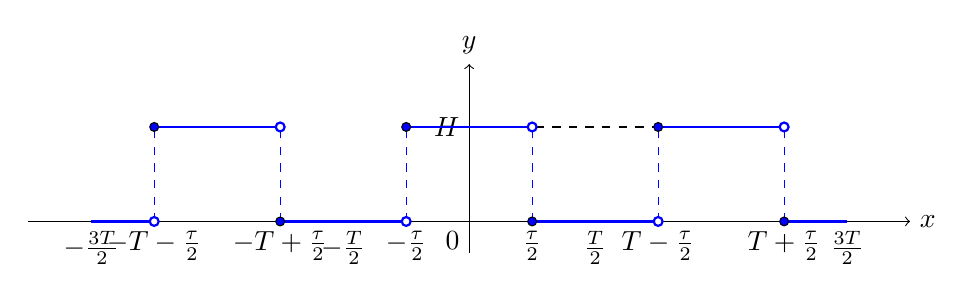
\begin{tikzpicture}[scale=0.8]
            % Axes
            \draw[->] (-7,0) -- (7,0) node[right] {$x$};
            \draw[->] (0,-0.5) -- (0,2.5) node[above] {$y$};

            % Labels on x-axis
            \node[below left] at (0,0) {$0$};
            \node[below] at (2,0) {$\frac{T}{2}$};
            \node[below] at (-2,0) {$-\frac{T}{2}$};
            \node[below] at (1,0) {$\frac{\tau}{2}$};
            \node[below] at (-1,0) {$-\frac{\tau}{2}$};

            \node[below] at (6,0) {$\frac{3T}{2}$};
            \node[below] at (-6,0) {$-\frac{3T}{2}$};
            \node[below] at (5,0) {$T+\frac{\tau}{2}$};
            \node[below] at (3,0) {$T-\frac{\tau}{2}$};
            \node[below] at (-5,0) {$-T-\frac{\tau}{2}$};
            \node[below] at (-3,0) {$-T+\frac{\tau}{2}$};

            % Label H on y-axis
            \node[left] at (0, 1.5) {$H$};
            \draw[dashed] (0, 1.5) -- (5, 1.5);

            % Draw the pulses
            % Period 0: [-T/2, T/2] -> [-2, 2]
            \draw[thick, blue] (-2, 0) -- (-1, 0);
            \draw[thick, blue] (-1, 1.5) -- (1, 1.5);
            \draw[thick, blue] (1, 0) -- (2, 0);

            % Period 1: [T/2, 3T/2] -> [2, 6]
            \draw[thick, blue] (2, 0) -- (3, 0);
            \draw[thick, blue] (3, 1.5) -- (5, 1.5);
            \draw[thick, blue] (5, 0) -- (6, 0);

            % Period -1: [-3T/2, -T/2] -> [-6, -2]
            \draw[thick, blue] (-6, 0) -- (-5, 0);
            \draw[thick, blue] (-5, 1.5) -- (-3, 1.5);
            \draw[thick, blue] (-3, 0) -- (-2, 0);

            % Continuous lines connecting segments are vertical dashed lines
            \draw[dashed, blue] (-1, 0) -- (-1, 1.5);
            \draw[dashed, blue] (1, 0) -- (1, 1.5);
            \draw[dashed, blue] (3, 0) -- (3, 1.5);
            \draw[dashed, blue] (5, 0) -- (5, 1.5);
            \draw[dashed, blue] (-3, 0) -- (-3, 1.5);
            \draw[dashed, blue] (-5, 0) -- (-5, 1.5);

            % Dots and open circles
            % x = -\tau/2
            \draw[fill=blue] (-1, 1.5) circle (2pt);
            \draw[fill=white, draw=blue, thick] (-1, 0) circle (2pt);

            % x = \tau/2
            \draw[fill=blue] (1, 0) circle (2pt);
            \draw[fill=white, draw=blue, thick] (1, 1.5) circle (2pt);

            % x = T - \tau/2
            \draw[fill=blue] (3, 1.5) circle (2pt);
            \draw[fill=white, draw=blue, thick] (3, 0) circle (2pt);

            % x = T + \tau/2
            \draw[fill=blue] (5, 0) circle (2pt);
            \draw[fill=white, draw=blue, thick] (5, 1.5) circle (2pt);

            % x = -T + \tau/2
            \draw[fill=blue] (-3, 0) circle (2pt);
            \draw[fill=white, draw=blue, thick] (-3, 1.5) circle (2pt);

            % x = -T - \tau/2
            \draw[fill=blue] (-5, 1.5) circle (2pt);
            \draw[fill=white, draw=blue, thick] (-5, 0) circle (2pt);
        \end{tikzpicture}
    \end{center}

    复数形式的 Fourier 级数展开式为
    \begin{equation}
        f(x) \sim \sum_{n=-\infty}^{\infty} c_n \e^{\ii n \omega_0 x}.
    \end{equation}

    计算复数 Fourier 系数：
    对于 $n = 0$：
    \begin{equation}
        c_0 = \frac{1}{T} \int_{-\frac{T}{2}}^{\frac{T}{2}} f(x) \d x = \frac{1}{T} \int_{-\frac{\tau}{2}}^{\frac{\tau}{2}} H \d x = \frac{H\tau}{T}.
    \end{equation}

    对于 $n \neq 0$：
    \begin{equation}
        \begin{aligned}
            c_n & = \frac{1}{T} \int_{-\frac{T}{2}}^{\frac{T}{2}} f(x) \e^{-\ii n \omega_0 x} \d x                               \\
                & = \frac{1}{T} \int_{-\frac{\tau}{2}}^{\frac{\tau}{2}} H \e^{-\ii n \omega_0 x} \d x                            \\
                & = \frac{H}{T} \left[ \frac{\e^{-\ii n \omega_0 x}}{-\ii n \omega_0} \right]_{-\frac{\tau}{2}}^{\frac{\tau}{2}} \\
                & = \frac{H}{T} \frac{\e^{-\ii n \omega_0 \frac{\tau}{2}} - \e^{\ii n \omega_0 \frac{\tau}{2}}}{-\ii n \omega_0} \\
                & = \frac{2H}{T n \omega_0} \sin\left( \frac{n \omega_0 \tau}{2} \right).
        \end{aligned}
    \end{equation}

    代入 $\omega_0 = \frac{2\uppi}{T}$ 得：
    \begin{equation}
        c_n = \frac{H}{n\uppi} \sin\left( \frac{n\uppi\tau}{T} \right).
    \end{equation}

    引进抽样函数 $\operatorname{sa}(u) = \frac{\sin u}{u}$（规定 $\operatorname{sa}(0) = 1$），则以上两式可统一表示为：
    \begin{equation}
        c_n = \frac{H\tau}{T} \operatorname{sa}\left( \frac{n\uppi\tau}{T} \right).
    \end{equation}

    因此，其 Fourier 级数的复数形式为
    \begin{equation}
        \boxed{f(x) \sim \sum_{n=-\infty}^{\infty} \frac{H\tau}{T} \operatorname{sa}\left( \frac{n\uppi\tau}{T} \right) \e^{\ii \frac{2n\uppi x}{T}}}.
    \end{equation}
\end{solution}

\endinput
